\chapter{Decomposition and Inertia Groups}
In this chapter we will study extra structure in the case when~$K$
is Galois over~$\Q$.   We will learn about Frobenius elements,
the Artin symbol, decomposition groups, and how the Galois group of
$K$ is related to Galois groups of residue class fields.  These are
the basic structures needed to attach $L$-function to representations of
$\Gal(\Qbar/\Q)$, which will play a central role in the next few
chapters.


\section{Galois Extensions}
In this section we give a survey (no proofs) of the basic facts about
Galois extensions of $\Q$ that will be needed in the rest of this
chapter.
\begin{definition}[Galois]
  An extension $K/L$ of number fields is \defn{Galois} if $$\#\Aut(K/L)
  = [K:L],$$ where $\Aut(K/L)$ is the group of automorphisms of $K$
  that fix $L$.  We write $$\Gal(K/L) = \Aut(K/L).$$
\end{definition}
For example, if $K\subset \C$ is a number field embedded in the complex numbers,
then $K$ is \defn{Galois} over $\QQ$ if
every field homomorphism $K\to \C$ has image $K$.
As another example, any quadratic extension
$K/L$ is Galois over $L$, since it is of the form $L(\sqrt{a})$, for some $a\in
L$, and the nontrivial automorphism is induced by $\sqrt{a}\mapsto
-\sqrt{a}$, so there is always one nontrivial automorphism.  If $f\in
L[x]$ is an irreducible cubic polynomial, and $a$ is a root of $f$,
then one proves in a course on Galois theory that $L(a)$ is Galois
over $L$ if and only if the discriminant of~$f$ is a perfect square
in~$L$.  ``Random'' number fields of degree bigger than $2$ are rarely
Galois.


If $K\subset \C$ is a number field, then the \defn{Galois closure} $K^{\gc}$
of $K$ in $\C$ is the field generated by all images of~$K$ under all
embeddings in~$\C$ (more generally, if $K/L$ is an extension, the
Galois closure of $K$ over $L$ is the field generated by images of
embeddings $K\to \C$ that are the identity map on $L$).  If $K=\Q(a)$,
then $K^{\gc}$ is the field generated by all of the conjugates of~$a$, and is
hence Galois over~$\Q$, since the image under an embedding of any
polynomial in the conjugates of~$a$ is again a polynomial in
conjugates of $a$.


How much bigger can the degree of $K^{\gc}$ be as compared to the
degree of $K=\Q(a)$? There is an embedding of
$\Gal(K^{\gc}/\Q)$ into the group of permutations of the conjugates of
$a$.  If $a$ has~$n$ conjugates, then this is an embedding
$\Gal(K^{\gc}/\Q)\hra S_n$, where $S_n$ is the symmetric group on~$n$
symbols, which has order~$n!$.  Thus the degree of the $K^{\gc}$ over~$\Q$
is a divisor of $n!$. Also $\Gal(K^{\gc}/\Q)$ is a transitive
subgroup of $S_n$, which constrains the possibilities further.  When
$n=2$, we recover the fact that quadratic extensions are Galois.  When
$n=3$, we see that the Galois closure of a cubic extension is either
the cubic extension or a quadratic extension of the cubic extension.
One can show that the Galois closure of a cubic extension is obtained
by adjoining the square root of the discriminant, which is why an
irreducible cubic defines a Galois extension if and only if the discriminant
is a perfect square.


For an extension
$K$ of $\QQ$ of degree $5$, it is ``frequently'' the case that the Galois
closure has degree $120$, and in fact it is an
interesting problem to enumerate examples of degree~$5$ extension in which
the Galois closure has degree smaller than $120$.
For example, the only possibilities for the order of a transitive proper subgroup
of $S_5$ are $5$, $10$, $20$, and $60$; there are also
proper subgroups of $S_5$ order $2, 3, 4, 6, 8, 12$, and $24$, but none
are transitive.

Let $n$ be a positive integer.  Consider the field $K=\Q(\zeta_n)$,
where $\zeta_n=e^{2\pi i/n}$ is a primitive $n$th root of unity.  If
$\sigma:K\to \C$ is an embedding, then $\sigma(\zeta_n)$ is also an
$n$th root of unity, and the group of $n$th roots of unity is cyclic,
so $\sigma(\zeta_n) = \zeta_n^m$ for some $m$ which is invertible
modulo $n$.  Thus $K$ is Galois and $\Gal(K/\Q)\hra (\Z/n\Z)^*$.
However, $[K:\Q]=\vphi(n)$, so this map is an isomorphism.  (Remark:
Taking a limit using the maps $\Gal(\Qbar/\Q)\to
\Gal(\Q(\zeta_{p^r})/\Q)$, we obtain a homomorphism $\Gal(\Qbar/\Q)\to
\Z_p^*$, which is called the {\em $p$-adic cyclotomic character}.)

Compositums of Galois extensions are Galois.  For example, the
biquadratic field $K=\Q(\sqrt{5},\sqrt{-1})$ is a Galois
extension of $\Q$ of degree~$4$, which is the compositum
of the Galois extensions $\Q(\sqrt{5})$ and $\Q(\sqrt{-1})$ of $\Q$.

Fix a number field $K$ that is Galois over a subfield
$L$. Then the Galois group $G=\Gal(K/L)$ acts on many
of the object that we have associated to $K$.

\begin{exercise}
	Describe the natural action of $G$ on the following objects:
	\begin{itemize}
		\item The ring of integers $\O_K$
		\item The group units $U_K$
		\item The set of ideals of $\O_K$
		\item The group of fractional ideals of $\O_K$
		\item The class group $\Cl(K)$
		\item The set $S_\p$ of prime ideals lying over a given nonzero
	prime ideal $\p$ of $\O_L$, i.e., the prime divisors of $\p\O_K$
	\end{itemize}
\end{exercise}

In the next section we will be concerned with the action of
$\Gal(K/L)$ on $S_\p$, though actions on each of the other objects,
especially $\Cl(K)$, are also of great interest.  Understanding the
action of $\Gal(K/L)$ on $S_{\p}$ will enable us to associate, in a
natural way, a holomorphic $L$-function to any complex representation
$\Gal(K/L) \to \GL_n(\C)$.

\section{Decomposition of Primes: $efg=n$}
If $I\subset \O_K$ is any ideal in the ring of integers of
a Galois extension $K$ of $\Q$ and $\sigma\in\Gal(K/\Q)$, then
$$
  \sigma(I) = \{\sigma(x) : x \in I\}
$$
is also an ideal of $\O_K$.


Fix a prime $\p\subset \O_K$ and write $\p\O_K = \P_1^{e_1}\cdots
\P_g^{e_g}$, so $S_\p=\{\P_1,\ldots, \P_g\}$.
\begin{definition}[Residue class degree]
Suppose $\P$ is a prime of $\O_K$ lying over $\p$.
Then the \defn{residue class degree} of $\P$ is
$$
   f_{\P/\p} = [\O_K/\P : \O_L/\p],$$
i.e., the degree of the extension of residue class fields.
\end{definition}
If $M/K/L$ is a tower of field extensions and
$\q$ is a prime of $M$ over $\P$, then
$$f_{\q/\p} = [\O_M/\q : \O_L/\p]
=[\O_M/\q : \O_K/\P]\cdot [\O_K/\P : \O_L/\p] =
f_{\q/\P}\cdot f_{\P/\p},$$
so the residue class degree is multiplicative in
towers.

Note that if $\sigma\in\Gal(K/L)$ and $\P\in S_p$, then $\sigma$
induces an isomorphism of finite fields $\O_K/\P\to \O_K/\sigma(\P)$
that fixes the common subfield $\O_L/\p$.  Thus the residue class
degrees of $\P$ and $\sigma(\P)$ are the same.  In fact, much more is
true.
\begin{theorem}\label{thm:transitive}\ithm{transitive Galois action}
Suppose $K/L$ is a Galois extension of number fields,
and let $\p$ be a prime of $\O_L$.  Write
$\p\O_K=\prod_{i=1}^g \P_i^{e_i}$, and let $f_i = f_{\P_i/\p}$.
Then
$G=\Gal(K/L)$ acts transitively on the set
$S_\p$ of primes $\P_i$, and
$$
  e_1=\cdots =e_g, \qquad f_1 =\cdots = f_g.
$$
Morever, if we let $e$ be the common value of the $e_i$,
$f$ the common value of the $f_i$, and $n=[K:L]$, then
$$
   efg=n.
$$
\end{theorem}
\begin{proof}
For simplicity, we will give the proof only in the case $L=\Q$, but
the proof works in general.  Suppose $p\in\Z$ and
$p\O_K=\p_1^{e_1}\cdots \p_g^{e_g}$, and $S=\{\p_1,\ldots, \p_g\}$.  We
will first prove that $G$ acts transitively on $S$.  Let $\p=\p_i$ for
some~$i$.   Recall Lemma~\ref{lem:magica} which we proved long ago using the
Chinese Remainder Theorem (Theorem~\ref{thm:crt}). It showed there exists
$a\in\p$ such that $(a)/\p$ is an integral ideal that is
coprime to $p\O_K$.   The product
\begin{equation}\label{eqn:prodquo}
 I= \prod_{\sigma\in G} \sigma((a)/\p)
   = \prod_{\sigma\in G} \frac{(\sigma(a))\O_K}{\sigma(\p)}
    = \frac{(\Norm_{K/\Q}(a))\O_K}{\displaystyle \prod_{\sigma\in G} \sigma(\p)}
\end{equation}
is a nonzero integral $\O_K$ ideal since it is a product of nonzero
integral $\O_K$ ideals.
Since $a\in \p$ we have that
$\Norm_{K/\Q}(a) \in \p\cap\Z=p\Z$.  Thus the numerator of
the rightmost expression in (\ref{eqn:prodquo}) is
divisible by $p\O_K$.   Also, because $(a)/\p$ is coprime
to $p\O_K$, each $\sigma((a)/\p)$ is coprime to $p\O_K$
as well.   Thus $I$ is coprime to $p\O_K$.   This means the
denominator of the rightmost expression in (\ref{eqn:prodquo})
must also be divisible by $p\O_K$ in order to cancel the $p\O_K$
in the numerator.  Thus we have shown that for any~$i$,
$$
  \prod_{j=1}^g \p_j^{e_j} = p\O_K \,\,\Big|\,\, \prod_{\sigma\in G} \sigma(\p_i).
$$
By unique factorization, since every $\p_j$ appears in the left hand
side, we must have that for each~$j$ there is a~$\sigma$ with
$\sigma(\p_i)=\p_j$, i.e., $G$ acts transitively on $S$.

Choose some $j$ and suppose that $k\neq j$ is another index.  Because
$G$ acts transitively, there exists $\sigma\in G$ such that
$\sigma(\p_k)=\p_j$.  Applying $\sigma$ to the factorization $p\O_K =
\prod_{i=1}^g \p_i^{e_i}$, we see that
$$\prod_{i=1}^g \p_i^{e_i} = \prod_{i=1}^g \sigma(\p_i)^{e_i}.$$
Using unique factorization,
we get $e_j = e_k$.  Thus $e_1=e_2=\cdots = e_g$.

As was mentioned right before the statement of the theorem,  for any $\sigma\in G$
we have $\O_K/\p_i\isom \O_K/\sigma(\p_i)$. Since $G$ acts transitively
it follows that $f_1=f_2=\cdots = f_g$.
We have, upon applying the Chinese Remainder Theorem
and noting $\#(\O_K/(\p^m)) = \#(\O_K/\p)^m$
(see Exercise~\ref{ex:residuefieldofpower}), that
\begin{align*}
[K:\Q]&= \dim_{\Z} \O_K = \dim_{\F_p} \O_K/p\O_K\\
    &= \dim_{\F_p} \left(\bigoplus_{i=1}^g \O_K/\p_i^{e_i}\right)
    = \sum_{i=1}^g e_i f_i
    = efg,
\end{align*}
which completes the proof.
\end{proof}

The rest of this section illustrates the theorem for quadratic fields
and a cubic field and its Galois closure.

\subsection{Special Cases}

\subsubsection*{Quadratic Extensions}

Suppose $K/\Q$ is a quadratic field.  Then $K$ is Galois, so for each prime $p\in\Z$ we have
$2=efg$. There are exactly three possibilities:
\begin{description}
\item[\bf{Ramified:}] $e=2$, $f=g=1$: The prime $p$ \emph{ramifies} in
$\O_K$, which means $p\O_K = \p^2$.  Let $\alpha$ be a generator for $\O_K$ and
$h\in\Z[x]$ a minimal polynomial for $\alpha$.
By Theorem~\ref{thm:fac1} a prime $p$ is ramified in $\O_K$ if and only if
$h$ has a double root modulo~$p$, which is equivalent to $p$ dividing
the discriminant of $h$. This shows there are only finitely many ramified
primes. More generally, the ramified primes are exactly the
ones that divide the discriminant (see \cite[Thm.~24]{marcus1977number}
or
\cite[Cor.~III.2.12]{neukirch1999}).

\item[\bf{Inert}:] $e=1$, $f=2$, $g=1$: The prime $p$ is \emph{inert} in $\O_K$,
which means $p\O_K = \p$ is prime.  It is a nontrivial theorem that
this happens half of the time,
as we will see illustrated below for a particular example.

\item[\bf{Split:}] $e=f=1$, $g=2$: The prime $p$ \emph{splits} in $\O_K$,
which means $p\O_K = \p_1\p_2$ with $\p_1\neq \p_2$.  This happens the other
half of the time.
\end{description}

\begin{example}\label{exam:decompQsqrt5}
Let $K=\Q(\sqrt{5})$, so $\O_K=\Z[\gamma]$, where
$\gamma=(1+\sqrt{5})/2$.  Then $p=5$ is ramified, since $5\O_K =
(\sqrt{5})^2$.  More generally, the order $\Z[\sqrt{5}]$ has index $2$
in $\O_K$, so for any prime $p\neq 2$ we can determine the
factorization of $p$ in $\O_K$ by finding the factorization of the
polynomial $x^2-5\in \F_p[x]$.  The polynomial $x^2-5$ splits as a
product of two distinct factors in $\F_p[x]$ if and only if $e=f=1$
and $g=2$.  For $p\neq 2,5$ this is the case if and only if $5$ is a
square in $\F_p$, i.e., if $\kr{5}{p} = 1$, where $\kr{5}{p}$ is $+1$
if $5$ is a square mod $p$ and $-1$ if $5$ is not.  By quadratic
reciprocity,
$$
 \kr{5}{p} = (-1)^{\frac{5-1}{2}\cdot \frac{p-1}{2}} \cdot \kr{p}{5} =
   \kr{p}{5} = \begin{cases} +1 & \text{ if } p\con \pm 1\pmod{5}\\ -1&\text{ if } p \con \pm 2\pmod{5}.\end{cases}
$$
Thus whether $p$ splits or is inert in
$\O_K$ is determined by the residue class of~$p$
modulo $5$.  It is a theorem of Dirichlet, which was massively
generalized by Chebotarev, that $p\con \pm 1$ half the time
and $p \con \pm 2$ the other half the time.\footnote{
For a technical statement and proof of this theorem,
see \cite{neukirch1999} Theorem~VII.13.4.}
\end{example}

\subsubsection*{The Cube Root of Two}

Suppose $K/\Q$ is not Galois.
Then $e_i$, $f_i$, and~$g$ are defined for each prime $p\in\Z$,
but we need not have $e_1=\cdots=e_g$ or $f_1=\cdots =f_g$.  We do still have that
$\sum_{i=1}^g e_i f_i = n$, by the Chinese Remainder Theorem.
For a proof of this identity, see \cite{marcus1977number} Theorem~$21$,
or, for a slightly more general version, \cite{neukirch1999} Proposition~I.8.2

Consider the case where $K=\Q(\sqrt[3]{2})$. We know that $\O_K = \Z[\sqrt[3]{2}]$.  Thus
$2\O_K = (\sqrt[3]{2})^3$, so for $2$ we have $e=3$ and $f=g=1$.

Working modulo $5$ we have
$$
 x^3 - 2 = (x+2)(x^2+3x+4) \in \F_5[x],
$$
and the quadratic factor is irreducible.  Thus
$$
 5\O_K = (5, \crtwo+2)\cdot (5, \crtwo^2 + 3\crtwo + 4).
$$
Thus here $g=2$, $e_1=e_2=1$, $f_1=1$, and $f_2=2$.
Thus when $K$ is not Galois we need not have that the $f_i$
are all equal.

\subsection{Definitions and Terminology}

In the previous sections we used words like ``ramify'',
``inert'', and ``split'' to describe the decomposition
of a prime in an extension. This section will define
the generalizations of these concepts which will be used
in later sections.

Let $K/L$ be an extension of number fields. Let
$\O_K,\O_L$ denote the respective ring of integers
and $\q$ a prime in $\O_L$. By Theorem~\ref{thm:intuniqfac} we
know that the ideal $\q\O_K$ factors uniquely into a product
of primes $\p_i$ in $\O_K$ given by
$$
\q\O_K = \p_1^{e_1}\cdots\p_g^{e_g}.
$$
Let $f_i$ be the degree of the extension of
residue fields, i.e.,
$$
f_i = [\O_K/\p_i : \O_L/\q].
$$

\begin{definition}\label{def:ramify}
	The prime $\q$ \emph{ramifies} in $L$
	if $e_i>1$ for some $1\leq i\leq g$.
	Otherwise $\q$ is \emph{unramified}.
	%in geneal, residue fields should be separable, neukrich 49
	If $\q$ is ramified and moreover $f_i=1$
	for all $i$, then $\q$ is \emph{totally ramified}.
\end{definition}

\begin{definition}\label{def:inert}
	The prime $\p$ is \emph{inert} in $L$
	if $\p\O_L$ is prime. In this case we have $g=1$,
	$\q_1=\p\O_L$, and $e_1=1$.
\end{definition}

\begin{definition}\label{def:split}
	The prime $\p$ is \emph{split} in $L$
	if $g>1$. If moreover $g = [L : K]$, then
	$\p$ \emph{splits completely} or is
	\emph{totally split}.
\end{definition}

It will sometimes be helpful to emphasize which prime we are
referring to. To do this we will use the notation $e(\p/\q)$
to represent the power of $\p$ appearing in the
factorization of $\q\O_K$. The number $e(\p/\q)$ is called the
\emph{ramification index} of $\p$ over $\q$.
In this notation we could write $\q\O_K = \prod \p^{e(\p/\q)}$
where the product ranges over all primes $\p$ in $\O_K$.
We will similarly denote $f(\p/\q)$ to be the degree of the extension
of residue fields $[\O_K/\p:\O_L/\q]$. The number $f(\p/\q)$ is called
the \emph{inertia degree} of $\p/\q$. Because the number of primes
over $\q$ depends on the field $K$, we sometimes denote $g$ by $g_K(\q)$.

\begin{exercise}\label{ex:ramificationmultiplicative}
The following are some basic properties of decompositions.
For each one, compare the result with previous examples
we have seen such as Example~\ref{exam:decompQsqrt5}.

Let $K/L/\Q$ be a tower of number fields. Let $p$ be a prime
in $\Z$, $\q$ a prime in $\O_L$ lying over $p$, and $\p$ a prime
in $\O_K$ lying over $\q$.
\begin{enumerate}
	\item[(a)] Show that $e$ is multiplicative, that is $e(\p/p)=e(\p/\q) \cdot e(\q/p)$.
	\item[(b)] Show that $f$ is multiplicative, that is $f(\p/p)=f(\p/\q) \cdot f(\q/p)$.
	\item[(c)] Let $g_L(p)$ be the number of primes of $\O_L$ lying over $p$.
	Show that $g_K(p) = \sum\limits_{\q \text{ lies over } p} g_L(\q)$.
\end{enumerate}
\end{exercise}

\begin{exercise}[See \cite{marcus1977number}, Chapter 4 problem 24]
Continue the notation from the previous exercise.
\begin{enumerate}
	\item[(a)]
	If $p$ it totally ramified in $K$
	then it is totally ramified in $L$.

	\item[(b)]
	Let $K'$ be another extension of $L$.
	If $\p$ is totally ramified in $K$ and unramified in $K'$
	then $K\cap K' = L$.
\end{enumerate}

\end{exercise}

\section{The Decomposition Group}
Suppose $K$ is a number field that is Galois over $\Q$ with
group $G=\Gal(K/\Q)$.
Fix a prime $\p\subset \O_K$ lying over $p\in\Z$.
\begin{definition}[Decomposition group]\label{def:decomp}
The \defn{decomposition group} of $\p$ is the subgroup
$$
  D_\p = \{\sigma \in G : \sigma(\p)=\p\} \subset G.
$$
\end{definition}
Note that $D_\p$ is the stabilizer of $\p$ for
the action of $G$ on the set of primes lying over $p$.

It also makes sense to define decomposition groups for relative
extensions $K/L$, but for simplicity and to fix ideas in this section
we only define decomposition groups for a Galois extension $K/\Q$.

Let $k_\p = \O_K/\p$ denote the residue class field of $\p$.
In this section we will prove that there is an exact sequence
$$
  1\to I_\p \to D_\p \to \Gal(k_{\p}/\F_p)\to 1,
$$
where $I_\p$ is the \defn{inertia subgroup} of $D_\p$, and
$\#I_\p=e = e(\p/p)$.
The most interesting part of the proof is
showing that the natural map $D_\p\to  \Gal(k_{\p}/\F_p)$
is surjective. We will also discuss the structure of $D_\p$ and introduce
Frobenius elements, which play a crucial role in understanding Galois
representations.


Recall from Theorem~\ref{thm:transitive}
that~$G$ acts transitively on the set of primes~$\p$ lying
over~$p$.  The orbit-stabilizer theorem implies that $[G:D_\p]$ equals the cardinality of the
orbit of~$\p$, which by Theorem~\ref{thm:transitive}
equals the number~$g$ of primes lying over~$p$, so $[G:D_\p]=g$.

\begin{lemma}\label{decompGpsConj}\ilem{decomposition groups are conjugate}
The decomposition subgroups $D_\p$ corresponding to primes $\p$
lying over a given $p$ are all conjugate as subgroups of~$G$.
\end{lemma}
\begin{proof}
See Exercise~\ref{ex:decompGpsConj}.
\end{proof}

\begin{exercise}\label{ex:decompGpsConj}
Prove Lemma~\ref{decompGpsConj}.

\begin{hint}
	For $\sigma,\tau\in G$ you need to show
	$\tau D_\p \tau^{-1} = D_{\tau\p}$.
	Start by writing down what it means for $\sigma\in D_\p$
	and $\tau\sigma\tau^{-1}\in D_{\tau\p}$.
\end{hint}

%solution:
%We have for each $\sigma, \tau \in G$, that
%$$\tau^{-1}\sigma \tau\p = \p
%\iff
%\sigma\tau \p = \tau \p,
%$$
%so
%$$
%\sigma \in D_{\tau\p} \iff \tau^{-1}\sigma\tau\in D_\p.
%$$
%Thus
%$$
% \sigma \in D_\p \iff \tau \sigma \tau^{-1} \in D_{\tau \p},
%$$
%which shows $\tau D_{\p}\tau^{-1} = D_{\tau \p}$.
\end{exercise}

The decomposition group is useful because it allows us
to refine the extension $K/\Q$ into a tower of extensions, such that at
each step in the tower we understand the splitting behavior
of the primes lying over~$p$.


Recall the correspondence between subgroups of the Galois group
$G$ and subfields of $K$. The fixed fields corresponding to the
decomposition and inertia subgroups have an important description
in terms of the splitting behavior of the prime $\p$.
We characterize the fixed field of $D=D_\p$ as follows.

\begin{proposition}\label{prop:nosplit}\iprop{fixed field characterization}
The fixed field
$$K^D=\{a \in K : \sigma(a) = a\text{ for all }
\sigma \in D\}$$
of $D$
is the smallest subfield $L\subset K$ such that
the prime ideal $\q = \p\cap\O_L$
has $g_K(\q)=1$, i.e., there is a unique
prime of $\O_K$ lying over $\q$.
\end{proposition}
\begin{proof}
First suppose $L=K^D$, and note that by Galois theory $\Gal(K/L)\isom
D$, and by Theorem~\ref{thm:transitive}, the group $D$
acts transitively on the primes of $K$ lying over $\q$.  One of
these primes is $\p$, and $D$ fixes $\p$ by definition, so there is
only one prime of $K$ lying over $\q$, that is $g=1$.
Conversely, if $L\subset K$ is such that $\q$
has $g=1$, then $\Gal(K/L)$ fixes $\p$ (since it is the only
prime over $\q$), so $\Gal(K/L)\subset D$, hence $K^D\subset L$.
\end{proof}

Thus $p$ does not split in going from $K^D$ to $K$---it does some
combination of ramifying and staying inert.  To fill in more of
the picture, the following proposition asserts that $p$ splits
completely and does not ramify in $K^D/\Q$.

\begin{proposition}\label{prop:noresidue}\iprop{$e$, $f$, $g$}
Fix a finite Galois extension~$K$ of~$\Q$,
let~$\p$ be a prime lying over~$p$ with decomposition group~$D$,
and set $L=K^D$ and $\q = \p \cap \O_L$.
Then $e(\q/p)=f(\q/p)=1$, $g_L(p)=[L : \Q]$, $e(\p/p)=e(\p/\q)$ and $f(\p/p)=f(\p/\q)$.
\end{proposition}
\begin{proof}
As mentioned right after Definition~\ref{def:decomp}, the
orbit-stabilizer theorem implies that $g_K(p)=[G:D]$, and
by Galois theory $[G:D]=[L:\Q]$, so $g_K(p) = [L:\Q]$. By
Proposition~\ref{prop:nosplit}, we have $g_K(\q)=1$ so
by Theorem~\ref{thm:transitive},
\begin{align*}
	e(\p/\q) \cdot f(\p/\q) = [K:L]
	&=\frac{[K:\Q]}{[L:\Q]} \\
	&= \frac{e(\p/p)\cdot f(\p/p) \cdot g_K(p)}{[L:\Q]}
	\\
	&= e(\p/p)\cdot f(\p/p).
\end{align*}
Now $e(\p/\q)\leq e(\p/p)$ and $f(\p/\q)\leq f(\p/p)$, so
we must have $e(\p/\q)=e(\p/p)$ and $f(\p/\q)=f(\p/p)$.
Since from Exercise~\ref{ex:ramificationmultiplicative} we have
$e(\p/p)=e(\p/\q)\cdot e(\q/p)$ and $f(\p/q)=f(\p/\q)\cdot f(\q/p)$,
it follows that $e(\q/p)=f(\q/p) = 1$.
\end{proof}

\noindent
We summarize the results of the decomposition of a prime
in the tower $K \supseteq L = K^D \supseteq \Q$ in
Table~\ref{tbl:decompfield}. This table shows the ramification
indices, inertia degrees, and the number of primes at each step
of the tower.

\begin{table}[h!]
\centering
\begin{tabular}{ >{$}c<{$} >{$}c<{$} >{$}c<{$} | >{$}c<{$} >{$}c<{$} }
	\text{Ramification ($e$)} & \text{Inertia ($f$)} & \text{Splitting ($g$)} & \text{Primes} & \text{Fields} \\
	\hline
	 &  &  & \p & K \\
	e(\p/p) & f(\p/p) & 1 & \vert & \vert \\
	 &  &  & \q & L \\
	1 & 1 & [L:\Q] & \vert & \vert \\
	 &  &  & p &  \Q
\end{tabular}
\caption{Decomposition in the fixed field $L=K^D$.}
\label{tbl:decompfield}
\end{table}

\subsection{Galois groups of finite fields}\label{sec:galoisfinite}

Each $\sigma\in D=D_\p$ acts in a well-defined
way on the finite field $k_{\p} = \O_K/\p$, so we obtain
a homomorphism
$$
  \vphi:D_\p \to \Aut(k_{\p}/\F_p).
$$
We pause for a moment and review a few basic properties of
extensions of finite fields. In particular, they turn out
to be Galois so the map $\vphi$ above is actually a map
$D_\p \to \Gal(k_{\p}/\F_p)$.
The properties in this section are general properties
of Galois groups for finite fields.

\begin{definition}
	Let $k$ be any field of characteristic $p$.
	Define $\Frob_p:k\to k$ to be the homomorphism
	given by $a\mapsto a^p$. The map $\Frob_p$ is
	called the \emph{Frobenius} homomorphism.
\end{definition}

\begin{exercise}\label{ex:frob}
\hfill
\begin{enumerate}
	\item[(a)]
	Show the map $\Frob_p$ is in fact a field homomorphism,
	that is $\Frob_p(a + b) = \Frob_p(a) + \Frob_p(b)$
	and $\Frob_p(ab) = \Frob_p(a)\Frob_p(b)$.
	
	\item[(b)]
	Suppose $k = \F_p$. Then show $\Frob_p = id$, i.e.,
	$a^p = a$ for any $a\in\F_p$.
	
	\item[(c)]
	Suppose $k = \F_{q}$ where $q=p^f$ for some $f\geq 1$. Show that $\Frob_p:k\to k$ is an automorphism.
	
	\item[(d)]
	Continuing part (c), note that by
	Exercise~\ref{ex:finitesubgroupoffieldcyclic}
	$k^*$ is cyclic. Let $a\in k$ be a generator for
	$k^*$, so $a$ has multiplicative order $p^f-1$ and $k = \F_p(a)$.
	Show that
	$$
	\Frob_p^n(a) = a^{p^n} = a
	\quad\Leftrightarrow\quad
	(p^f - 1) \mid p^n - 1
	\quad\Leftrightarrow\quad
	f \mid n
	$$
\end{enumerate}
\end{exercise}

\begin{remark}
	Exercise~\ref{ex:frob} shows that all finite fields
	are \emph{perfect}. For more on perfect fields see
	a standard abstract algebra text such as
	\cite{dummit2004abstract}.
\end{remark}

By Exercise~\ref{ex:frob}(b,c) the map $\Frob_p$ is an
automorphism of $k_\p$ fixing $\F_p$ and hence defines
an element in $\Gal(k_{\p}/\F_p)$. Let $f = f_{\p/p}$ be the residue
degree of $\p$, i.e., $f = [k_{\p}:\F_p]$.
Exercise~\ref{ex:frob}(d) shows the order of $\Frob_p$ is~$f$.
Since the order of the automorphism group of a field extension
is at most the degree of the extension, we conclude that
$\Aut(k_{\p}/\F_p)$ is generated by $\Frob_p$. This shows
$\Aut(k_{\p}/\F_p)$ has order equal to the degree $[k_{\p}/\F_p]$
so we conclude that $k_{\p}/\F_p$ is Galois.
We summarize the discussion into the following theorem.

\begin{theorem}\label{thm:galoisgroupfinitefield}
	The extension $k_{\p}/\F_p$ is Galois and moreover,
	$\Gal(k_{\p}/\F_p)$ is generated by the Frobenius map
	$\Frob_p$ defined by $a\mapsto a^p$.
\end{theorem}

\begin{exercise}
	Prove that up to isomorphism there is
	exactly one finite field of each degree.
	
	\begin{hint}
		By Theorem~\ref{thm:galoisgroupfinitefield}
		all elements in a finite field satisfy an equation
		of the form $x^{p^f} - 1$ where $p$ is the
		characteristic and $f$ is the degree over the
		field $\F_p$.
	\end{hint}
\end{exercise}


\subsection{The Exact Sequence}\label{sec:exactseq}
Because $D_\p$ preserves $\p$, there is a natural reduction homomorphism
$$
  \vphi:D_\p \to \Gal(k_{\p}/\F_p).
$$
\begin{theorem}\label{thm:redsurj}\ithm{reduction of Galois group}
The homomorphism $\vphi$ is surjective.
\end{theorem}
\begin{proof}
Let $D = D_\p$ and $\tilde{a} \in  k_{\p}$ be an element such that $ k_{\p} = \F_p(\tilde{a})$.
Lift $\tilde{a}$ to an algebraic integer $a\in \O_K$, and let
$h=\prod_{\sigma\in {D}}(x-\sigma(a))\in K^D[x]$.
Let $\tilde{h}$ be the reduction of $h$ modulo~$\p$.
Note that $h(a) = 0$ so $\tilde{h}(\tilde{a}) = 0$.

Note that the coefficients of $h$ lie in $\O_{K^D}$.
By Proposition~\ref{prop:noresidue}, the residue field of $\O_{K^D}$
is $\F_p$ so $\tilde{h}\in\F_p[x]$.
Therefore $\tilde{h}$ is a multiple of the minimal polynomial of
$\tilde{a}$ over $\F_p$. In particular, $\Frob_p(\tilde{a})$
must also be a root of $\tilde{h}$.
Since the roots of $\tilde{h}$ are of the form
$\widetilde{\sigma(a)}$ this shows that
$\widetilde{\sigma(a)} = \Frob(\tilde{a})$ for some $\sigma\in D$.
Hence $\varphi(\sigma)(\tilde{a}) = \Frob(\tilde{a})$. Since elements
of $\Gal(K_\p/\F_p)$ are determined by their action on $\tilde{a}$
by choice of $\tilde{a}$, it follows that $\vphi(\sigma) = \Frob$
and hence $\varphi$ is surjective because $\Frob_p$
generates $\Gal(k_\p/\F_p)$.
\end{proof}

\begin{definition}[Inertia Group]
The \defn{inertia group associated to
 $\p$} is the kernel $I_\p$ of $D_\p\to\Gal(k_{\p}/\F_p)$.
\end{definition}
We have an exact sequence of groups
\begin{equation}\label{eqn:exact}
   1 \to I_\p \to D_\p \to \Gal(k_{\p}/\F_p)\to 1.
\end{equation}
The inertia group is a measure of how $p$ ramifies in $K$.
\begin{corollary}\icor{order of inertia group}
We have $\# I_\p = e = e(\p/p)$.
\end{corollary}
\begin{proof}
The exact sequence (\ref{eqn:exact}) implies that
$\#I_\p = \#D_\p / f$ where $f = f(\p/p) = [k_\p : \F_p]$.
Applying Propositions~\ref{prop:nosplit} and \ref{prop:noresidue}, we have
$$\#D_\p = [K:L] = \frac{[K:\Q]}{g} = \frac{efg}{g} = ef.$$
Dividing both sides by $f$ proves the corollary.
\end{proof}

We have the following characterization of $I_\p$.
\begin{proposition}\label{prop:charip}\iprop{inertia group characterization}
Let $K/\Q$ be a Galois extension with group $G$,
and let~$\p$ be a prime of $\O_K$ lying
over a prime~$p$.  Then
$$
I_\p = \{\sigma\in G \, :\, \sigma(a) \equiv a\pmod{\p}\text{ for all } a\in\O_K\}.
$$
\end{proposition}
\begin{proof}
  By definition $I_\p = \{\sigma\in D_\p : \sigma(a) \equiv
  a\pmod{\p}\text{ for all } a\in\O_K\}$, so it suffices to show that
  if $\sigma\not\in D_\p$, then there exists $a\in\O_K$ such that
  $\sigma(a)\not\con a\pmod{\p}$.  If $\sigma\not\in D_\p$, then
  $\sigma^{-1}\not\in D_\p$, so $\sigma^{-1}(\p)\neq \p$.  Since both
  are maximal ideals, there exists $a\in\p$ with
  $a\not\in\sigma^{-1}(\p)$, i.e., $\sigma(a)\not\in\p$.  Thus
  $\sigma(a)\not\con a\pmod{\p}$.
\end{proof}

%\begin{figure}\label{fig}
%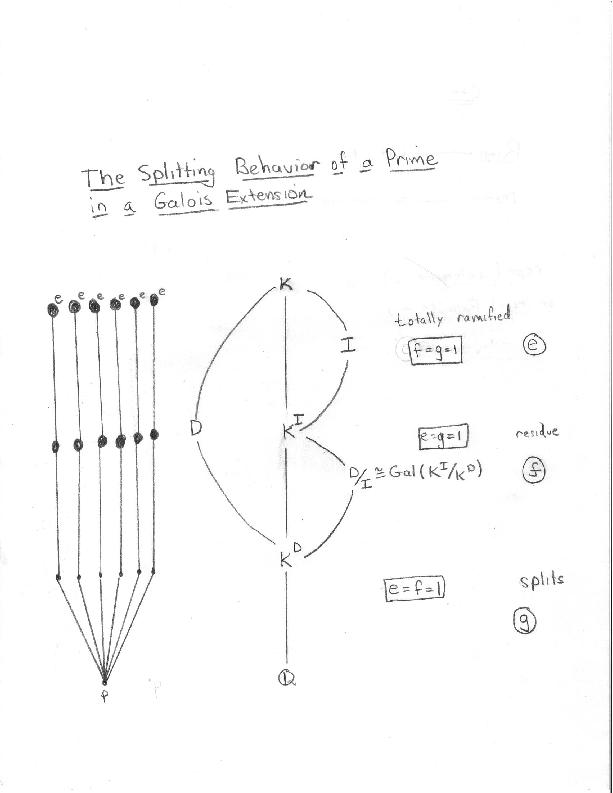
\includegraphics[width=\textwidth]{splitting}
%\caption{The Splitting of Behavior of a Prime in a Galois Extension}
%\end{figure}


\section{Frobenius Elements}

Suppose that $K/\Q$ is a finite Galois extension with group $G$ and
$p$ is a prime such that $e=1$ (i.e., an unramified prime).  Then
$I=I_\p=1$ for any $\p\mid p$, so the map $\vphi$ of
Theorem~\ref{thm:redsurj}
is a canonical isomorphism $D_\p \isom \Gal( k_{\p}/\F_p)$.
By Section~\ref{sec:galoisfinite},
the group $\Gal( k_{\p}/\F_p)$ is
cyclic with canonical generator $\Frob_p$.
The \defn{Frobenius element} corresponding to $\p$ is
$\Frob_\p\in D_\p$. It is the unique (see Exercise~\ref{ex:frobunique})
element of $G$ such that for all
$a\in\O_K$ we have
$$
  \Frob_\p(a)\con a^p\pmod{\p}.
$$


\begin{exercise}\label{ex:frobunique}
	With the notation above, prove that $\Frob_\p$ is
	unique. That is, if $\sigma$ satisfies
	$\sigma(a) \equiv a^p \pmod{\p}$ for all $a\in\O_K$
	then $\sigma = \Frob_\p$.

	\begin{hint}
		First show $\sigma\in D_\p$, then argue as in
		the proof of Proposition~\ref{prop:charip}.
	\end{hint}
\end{exercise}


Just as the primes $\p$ and decomposition groups $D_\p$ are all
conjugate, the Frobenius elements corresponding to primes
$\p\mid p$ are all conjugate as elements of~$G$.

\begin{proposition}\iprop{conjugation of Frobenius}
For each $\sigma \in G$, we have
$$
 \Frob_{\sigma\p} = \sigma\Frob_\p\sigma^{-1}.
$$
In particular, the Frobenius elements lying over a given
prime are all conjugate.
\end{proposition}
\begin{proof}
Fix $\sigma\in G$. For any $a\in\O_K$ we have
$\Frob_\p(\sigma^{-1}(a)) - \sigma^{-1}(a)^p \in \p$.
Applying~$\sigma$ to both sides, we see that
$\sigma\Frob_\p(\sigma^{-1}(a)) - a^p \in \sigma\p$,
so $\sigma\Frob_\p\sigma^{-1} = \Frob_{\sigma \p}$.
\end{proof}

Thus the conjugacy class of $\Frob_\p$ in $G$ is a well-defined
function of~$p$.  For example, if $G$ is abelian, then $\Frob_\p$ does
not depend on the choice of $\p$ lying over $p$ and we obtain a well
defined symbol $\kr{K/\Q}{p} =\Frob_\p\in G$ called the \defn{Artin
symbol}.  It extends to a homomorphism from the free abelian
group on unramified primes~$p$ to~$G$.
Class field theory (for~$\Q$) sets up a natural bijection
between abelian Galois extensions of $\Q$ and certain maps from
certain subgroups of the group of fractional ideals for~$\Z$ (i.e., $\Q^*$).
  We have
just described one direction of this bijection, which associates to an
abelian extension the Artin symbol (which is a homomorphism).
The Kronecker-Weber theorem asserts that the abelian extensions of
$\Q$ are exactly the subfields of the fields $\Q(\zeta_n)$, as $n$
varies over all positive integers.  By Galois theory there is a
correspondence between the subfields of the field $\Q(\zeta_n)$,
which has Galois group $(\Z/n\Z)^*$, and the subgroups of $(\Z/n\Z)^*$.
If $H \subseteq (\Z/n\Z)^*$ is the subgroup corresponding to
$K \subset \Q(\zeta_n)$ then the Artin reciprocity map
$p\mapsto \kr{K/\Q}{p}$ is given by $p\mapsto [p]\in (\Z/n\Z)^*/H$.

\begin{remark}
	Notice above that the $n$ used is not unique. That is,
	if~$K$ is an abelian extension of $\Q$ then it lies in some~$\Q(\zeta_n)$.
	But then it also lies inside of~$\Q(\zeta_{dn})$ for any
	positive integer~$d$. However, a different choice of $n$
	would mean a different choice of $H$. Note that the
	quotient $(\Z/n\Z)^*/H$ used is not dependent on $n$
	since it is isomorphic to the Galois group of $K/\Q$.
\end{remark}

\section{The Artin Conjecture}\label{sec:artin}

The Galois group $\Gal(\Qbar/\Q)$ is an object of central importance
in number theory, and we can interpret much of number theory as the
study of this group.  A good way to study a group is to study how it
acts on various objects, that is, to study its representations.

Endow $\galq$ with the topology which has as a basis of open neighborhoods
of the origin the subgroups $\Gal(\Qbar/K)$, where~{$K$ varies
over finite Galois extensions of~$\Q$.
Fix a positive integer~$n$ and let $\GL_n(\C)$ be the group of
$n\times n$ invertible matrices over~$\C$ with the discrete topology.

\begin{warning}\label{warn:galqtopology}
	The topology on $\galq$ is {\bf not} the topology induced
	by taking as a basis of open neighborhoods around the origin
	the collection of finite-index normal subgroups of $\galq$,
	see \cite[Chapter 7]{milne:FT} or
	Exercise~\ref{ex:nonopensbgpfiniteindexgalq}. In particular,
	there exist nonopen normal subgroups of finite index which
	do not correspond to subgroups $\Gal(\Qbar/K)$ for some
	finite Galois extension $K/\Q$.
\end{warning}

\begin{definition}
A \defn{complex  $n$-dimensional representation} of $\galq$
is a continuous homomorphism
$$
  \rho:\galq\to \GL_n(\C).
$$
\end{definition}
For $\rho$ to be continuous means that if $K$ is the fixed
field of $\Ker(\rho)$, then $K/\Q$ is a finite Galois extension.  We have
a diagram
$$\xymatrix{ {\galq}\ar[rr]^{\rho}\ar[dr]& &{\GL_n(\C)}\\
&{\Gal(K/\Q)}\ar@{^{(}->}[ur]_{\rho'}}
$$

\begin{exercise}\label{ex:galqrepfiniteimage}
	Suppose $\rho:\galq\to\GL_n(\C)$ is continuous.
	Show that the image is finite.
\end{exercise}

\begin{remark}
	The converse to Exercise~\ref{ex:galqrepfiniteimage}
	is \textbf{false} in general (see
	Exercise~\ref{ex:nonopensbgpfiniteindexgalq}).
	This is essentially the same warning as
	\ref{warn:galqtopology}, however it is worth
	pointing out to avoid mistakes.
	\footnote{See \cite[p. 1]{artinconjectureLectureNotes}.}
\end{remark}

\begin{exercise}\label{ex:nonopensbgpfiniteindexgalq}
	Find a nonopen subgroup of index $2$ in $\galq$.
	Note this is also an example of a non-continuous
	homomorphism $\galq\to\GL_n(\C)$ with finite image.
	
	
	\begin{hint}
		Use Zorn's lemma to show that there are homomorphisms
		$\galq\to\{\pm 1\}$ with finite image that are not continuous,
		since they do not factor through the Galois group of any
		finite Galois extension.
	\end{hint}
	
	\begin{hint}
		The extension $\Q(\sqrt{d}, d \in \Q^*/(\Q^*)^2)$
		is an extension of~$\Q$ with Galois group $X\ncisom \prod \F_2$.
		The index-two open subgroups of~$X$ correspond to the quadratic
		extensions of~$\Q$. However, Zorn's lemma implies that~$X$
		contains many index-two subgroups that do not correspond to
		quadratic extensions of~$\Q$.
	\end{hint}
\end{exercise}

Fix a Galois representation~$\rho$ and let $K$ be the fixed field of
$\ker(\rho)$, so~$\rho$ factors through $\Gal(K/\Q)$.  For each prime
$p\in\Z$ that is not ramified in $K$, there is an element
$\Frob_\p\in\Gal(K/\Q)$ that is well-defined up to conjugation by
elements of $\Gal(K/\Q)$.  This means that $\rho'(\Frob_p)\in
\GL_n(\C)$ is well-defined up to conjugation.  Thus the characteristic
polynomial $F_p(x)\in\C[x]$ of $\rho'(\Frob_p)$ is a well-defined
invariant of $p$ and $\rho$.  Let
$$R_p(x) = x^{\deg(F_p)}\cdot F_p(1/x) = 1 + \cdots +
\det(\Frob_p)\cdot x^{\deg(F_p)}$$
be the polynomial obtain
by reversing the order of the coefficients of $F_p$.
Following E.~Artin \cite{artin:conjecture, artin:conjecture2}, set
\begin{equation}\label{eqn:artin}
L(\rho,s) = \prod_{p\text{ unramified}}
\frac{1}{R_p(p^{-s})}.
\end{equation}
We view $L(\rho,s)$ as a function of a single complex variable $s$.
One can prove that $L(\rho,s)$ is holomorphic on some right
half plane, and extends to a meromorphic function on all $\C$.
\begin{conjecture}[Artin]\label{conj:artin}
The $L$-function of any continuous representation $$\Gal(\Qbar/\Q)\to\GL_n(\C)$$
is an entire function on all $\C$, except possibly at $1$.
\end{conjecture}
This conjecture asserts that there is some way to analytically continue
$L(\rho,s)$ to the whole complex plane, except possibly at $1$.
(A standard fact from complex analysis is that this analytic
continuation must be unique.)
The simple pole at $s=1$ corresponds to the trivial representation (the
Riemann zeta function), and if $n\geq 2$ and $\rho$ is irreducible,
then the conjecture is that $\rho$ extends to a holomorphic function
on all $\C$.

The conjecture is known when $n=1$.  Assume for the rest of this
paragraph that $\rho$ is odd, i.e., if $c\in\Gal(\Qbar/\Q)$ is complex
conjugation, then $\det(\rho(c))=-1$.  When $n=2$ and the image of
$\rho$ in $\PGL_2(\C)$ is a solvable group, the conjecture is known,
and is a deep theorem of Langlands and others (see
\cite{langlands:basechange}), which played a crucial roll in Wiles's
proof of Fermat's Last Theorem.  When $n=2$ and the image of $\rho$ in
$\PGL_2(\C)$ is not solvable, the only possibility is that the
projective image is isomorphic to the alternating group~$A_5$.
Because~$A_5$ is the symmetry group of the icosahedron, these
representations are called \defn{icosahedral}.  In this case, Joe
Buhler's Harvard Ph.D. thesis \cite{buhler:thesis} gave the first
example in which $\rho$ was shown to satisfy
Conjecture~\ref{conj:artin}.  There is a book \cite{mr95i:11001},
which proves Artin's conjecture for 7 icosahedral representation (none
of which are twists of each other).  Kevin Buzzard and the author
proved the conjecture for 8 more examples \cite{buzzard-stein:artin}.
Subsequently, Richard Taylor, Kevin Buzzard, Nick Shepherd-Barron, and
Mark Dickinson proved the conjecture for an infinite class of
icosahedral Galois representations (disjoint from the examples)
\cite{bdsbt}.  The general problem for $n=2$ is in fact now completely
solved, due to recent work of Khare and Wintenberger
\cite{khare-wintenberger:serre1} that proves Serre's conjecture.

%%% Local Variables:
%%% mode: latex
%%% TeX-master: "ant"
%%% End:
